\section{Qualidade do Código Fonte}

\subsection{SonarQube}

\begin{figure}[H]

  \centering

  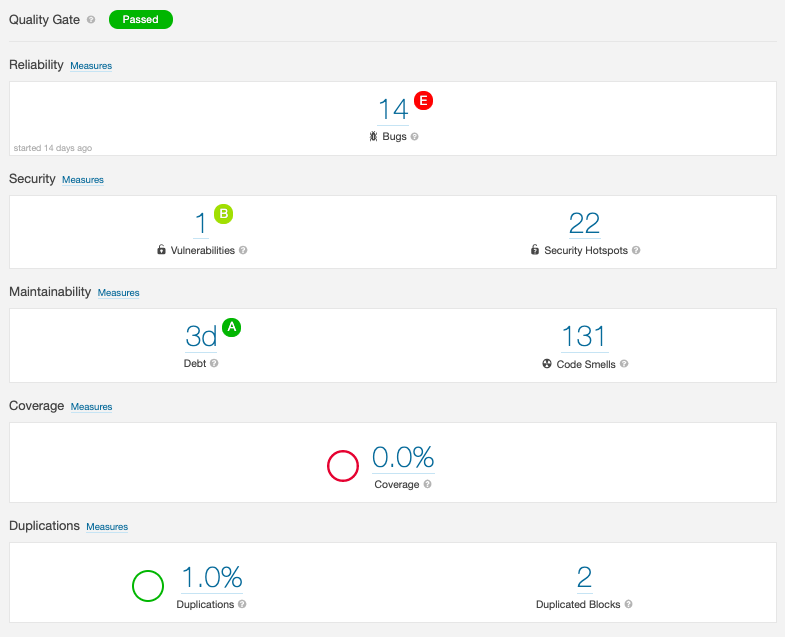
\includegraphics[scale = 0.5]{sonarEvaluation.png}

  \caption {Menu geral de avaliação do SonarQube}

  \label {fig01}

\end{figure}


\par Como se pode ver pela figura~\ref{fig:fig01} este projeto possui alguns bugs, pelo menos 1 vulnerabilidade uma quantidade consideravel de code smells e 2 blocos duplicados.


De seguida apresenta-se um relatório detalhado dos tipos de erros e da sua gravidade:
\subsection{Bugs}
versão com bugs, sem bugs, com smells sem smells (por tipos de smells) -> descriminar o impacto dos smells
\subsubsection{Blocker Bugs:}
\begin{itemize}
\item Não usar blocos try/catch ao ler um ficheiro.\newline
resolução....
\item Não usar blocos try/catch ao escrever em ficheiros.\newline
\end{itemize}

\subsubsection{Critical Bugs:}
\begin{itemize}
\item Guardar e reutilizar variáveis random. \newline

\end{itemize}

\subsubsection{Major Bugs:}
\begin{itemize}
\item Não obrigar a usar o método redifinido usando override.\newline


.................Rever...............
\par Para resolver este problema fo preciso definir a função isEqual, visto que usando um \textit{@Override} este método obrigaria a implementar um método do super tipo.

\end{itemize}

\subsubsection{Minor Bugs:}
\begin{itemize}
\item Obrigar o override do equals e não do método hashCode().\newline
\end{itemize}


\subsection{Vulnerabilitys}
\begin{itemize}
\item Utilizar printStackTrace() pode revelar informação sensivel.\newline
\end{itemize}

\subsection{CodeSmells}

\begin{itemize}
\item Blocos de código repetidos.\newline
\end{itemize}





